\documentclass[twoside,11pt]{article}


% Any additional packages needed should be included after jmlr2e.
% Note that jmlr2e.sty includes epsfig, amssymb, natbib and graphicx,
% and defines many common macros, such as 'proof' and 'example'.
%
% It also sets the bibliographystyle to plainnat; for more information on
% natbib citation styles, see the natbib documentation, a copy of which
% is archived at http://www.jmlr.org/format/natbib.pdf
\usepackage{ctex}
%\usepackage{jmlr2e}
\usepackage{amsmath}
\newtheorem{myDef}{Definition}
\newtheorem{myTheo}{Theorem}
\newtheorem{myCor}{Corollary}
\newtheorem{myProp}{Proposition}
\usepackage{graphicx}
\usepackage{caption}
\usepackage{AMSFonts}
\usepackage{amsfonts}
\usepackage{subfigure}
% Definitions of handy macros can go here

\newcommand{\dataset}{{\cal D}}
\newcommand{\fracpartial}[2]{\frac{\partial #1}{\partial  #2}}

% Heading arguments are {volume}{year}{pages}{submitted}{published}{author-full-names}

%
%% Short headings should be running head and authors last names
%
%\ShortHeadings{Bayesian graphical model}
%\firstpageno{1}
%\input{notation.tex}
\begin{document}
\section{NYSE data Analysis}
\noindent First we plot the data with timing diagram:
\begin {figure}[h]
\centering
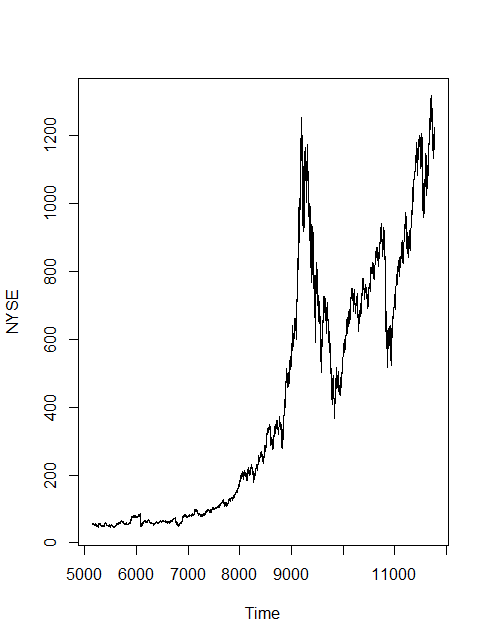
\includegraphics[width=8cm,height=6cm]{NYSE.png}
\end {figure}

\noindent Intuitively, the data is not stationary, not to mention white noise.\\
\\
\noindent \textbf{1}. Make the data be stationary with curve-fittin.\\ 
We use $e^{a_0+a_1x+a_2x_2}$ to fit the data, and get the coefficients.
\begin{verbatim}
> fit <- lm(log(NYSE) ~ x+I(x^2))
> fit
Call:
lm(formula = log(NYSE) ~ x + I(x^2))
Coefficients:
(Intercept)            x       I(x^2)
3.482e+00    6.837e-04   -1.793e-08
\end{verbatim}

We plot the stationary timing diagram:\\

\begin {figure}[h]
\centering
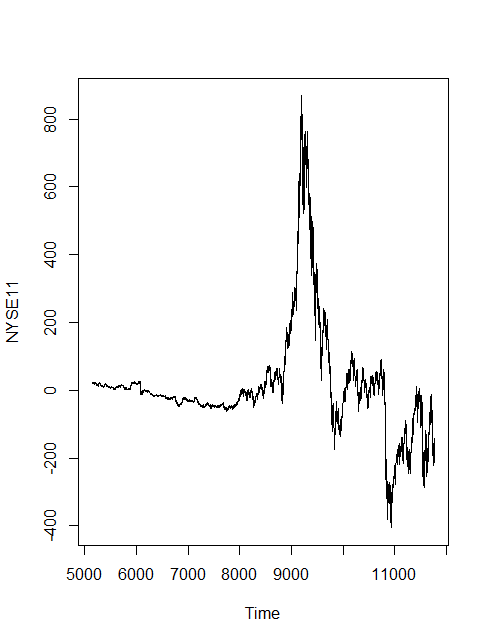
\includegraphics[width=8cm,height=6cm]{NYSE11.png}
\end {figure}

\noindent \textbf{2}.White noise test.\\ 
We conduct Ljung-Box white noise test to the transformed data.

\begin{verbatim}
> Box.test(NYSE11, type="Ljung-Box")
Box-Ljung test
data:  NYSE11
X-squared = 6603, df = 1, p-value < 2.2e-16
\end{verbatim}

\noindent We can see that the transformed data is significantly not white noise.\\
\\
\noindent \textbf{3}.Stationarity test.\\
Now we check if the transformed data is stationary.

\begin{verbatim}
> adf.test(NYSE11)
Augmented Dickey-Fuller Test
data:  NYSE11
Dickey-Fuller = -2.1416, Lag order = 18, p-value = 0.5184
alternative hypothesis: stationary
\end{verbatim}

So the transformed data is stationary, but obviously there is ARCH effect in the data. First, we can routinely build a linear time series model, for example the ARMA model. Then we consider to construct an appropriate ARCH model for the residue.\\

\noindent \textbf{4}. Build an ARMA model.\\
The notation ARMA $(p, q)$ refers to the model with $p$ autoregressive terms and $q$ moving-average terms. This model contains the $A R(p)$ and $M A(q)$ models
\[
X_{t}=c+\varepsilon_{t}+\sum_{i=1}^{p} \varphi_{i} X_{t-i}+\sum_{i=1}^{q} \theta_{i} \varepsilon_{t-i}
\]\\
$\mu$ is the expectation of $X_{t}$ (often assumed to equal 0), and the $\{\epsilon_t\}$ are white noise error terms.

\begin{verbatim}
> AIC1
[,1]     [,2]     [,3]     [,4]     [,5]     [,6]
[1,] 86578.60 77918.08 71176.67 66173.04 62871.84 60454.85
[2,] 49131.47 49133.12 49118.84 49117.01 49118.07 49111.59
[3,] 49133.20 49134.51 49115.36 49117.32 49119.06 49107.72
[4,] 49118.72 49115.68 49103.09 49108.64 49109.38 49112.41
[5,] 49117.96 49118.20 49102.68 49126.17 49105.92 49092.57
[6,] 49118.78 49119.44 49099.98 49093.22 49052.37 49113.43
\end{verbatim}
\noindent where AIC1[j,k] means the AIC value of model ARMA(j-1,k-1), and ARMA(5,4) is the best choice accordingly.\\
The corresponding coefficients:
\begin{verbatim}
> fit1
Call:
arima(x = NYSE11, order = c(5, 0, 4))
Coefficients:
     ar1   ar2     ar3    ar4   ar5   ma1   ma2   ma3   ma4   intercept
     -0.48 -0.58   0.605  0.495 0.952 1.491 2.05  1.43  0.945 14.71
s.e. 0.015  0.0102 0.0072 0.009 0.014 0.015 0.021 0.020 0.014 69.547
sigma^2 estimated as 95.8:  log likelihood = -24516.19,  aic = 49052.37
\end{verbatim}

\noindent (1).White noise test for ARMA model residual:
\begin{verbatim}
> Box.test(fit1$residuals, type="Ljung-Box") 
Box-Ljung test
data:  fit1$residuals
X-squared = 1.1988, df = 1, p-value = 0.2736
\end{verbatim}
Hence we do not reject that the residual of ARMA(5,4) model is white noise.\\

\noindent (2).The significance test for coefficients of ARMA(5,4).
\begin{verbatim}
> U1<-fit1$coef/sqrt(diag(fit1$var.coef)) #显著
> pnorm(abs(U1),0,1,lower.tail = FALSE)*2
ar1           ar2           ar3           ar4           ar5                 
1.381040e-217  0.000000e+00  0.000000e+00  0.000000e+00  0.000000e+00
ma1           ma2           ma3           ma4     intercept
0.000000e+00   0.000000e+00  0.000000e+00  0.000000e+00  8.325419e-01
\end{verbatim}

So the coefficients are viewed as significient.\\

\noindent (3).The ARCH effect of the residual of ARMA(5,4):\\
We plot the ARMA residuals with timing diagram:
\begin {figure}[h]
\centering
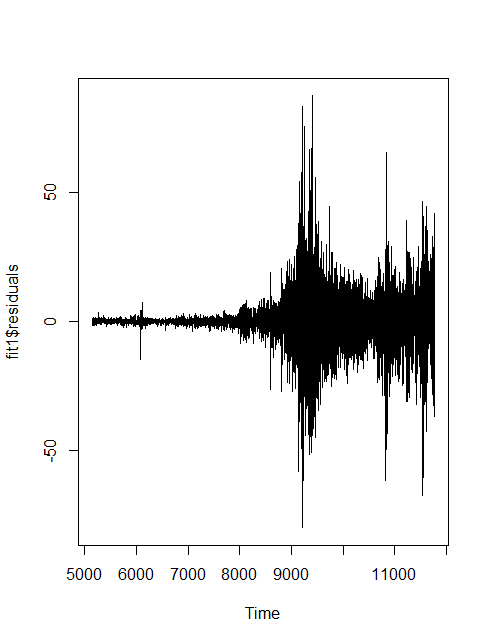
\includegraphics[width=8cm,height=6cm]{NYSE_res1.png}
\end {figure}
\noindent Obviously we can observe the ARCH effect, we examine it with a test.
\begin{verbatim}
> NYSE2<-fit1$residuals
> ArchTest(NYSE2)
ARCH LM-test; Null hypothesis: no ARCH effects
data:  NYSE2
Chi-squared = 1897, df = 12, p-value < 2.2e-16
\end{verbatim}
So the ARCH effect is very significent.\\
\\
\noindent \textbf{5}. Build a model for the residuals of ARMA(5,4):\\
ARCH model:\\
Assume $\epsilon_{t}=\sigma_{t} z_{t},$ where $z_{t} \overset{iid}\sim  N(0,1)$, The model of $\sigma_{t}$ is
$\sigma_{t}^{2}=\alpha_{0}+\alpha_{1} \varepsilon_{t-1}^{2}+\cdots+\alpha_{p} \varepsilon_{t-p}^{2}.$

If we apply the idea of ARMA to model $\sigma_{t}^{2}$, we get GARCH model:\\
$\sigma_{t}^{2}=\alpha_{0}+\alpha_{1} \varepsilon_{t-1}^{2}+\cdots+\alpha_{q} \varepsilon_{t-q}^{2}+\beta_{1} \sigma_{t-1}^{2}+\cdots+\beta_{p} \sigma_{t-p}^{2}.$\\

So we consider GARCH model. In fact, GARCH(1,1) is simple and efficient. The cofficients of GARCH(1,1):
\begin{verbatim}
> fit2<-garch(x=NYSE2 , order=c(1,1), trace = FALSE)
> fit2
Call:
garch(x = NYSE2, order = c(1, 1), trace = FALSE)
Coefficient(s):
a0        a1        b1
0.007149  0.099418  0.907365  
\end{verbatim}
(1).White noise test for the residual of GARCH(1,1) model:
\begin{verbatim}
Box-Ljung test
data:  Squared.Residuals
X-squared = 0.16209, df = 1, p-value = 0.6872
\end{verbatim}
\noindent So we view the residual of GARCH(1,1) as white noise.\\

\noindent (2).The significance test for coefficients of GARCH(1,1):
\begin{verbatim}
Coefficient(s):
Estimate  Std. Error  t value Pr(>|t|)
a0  0.007149    0.000919    7.779 7.33e-15 ***
a1  0.099418    0.003436   28.934  < 2e-16 ***
b1  0.907365    0.003076  294.986  < 2e-16 ***
\end{verbatim}
So the coefficients are significant.\\

\noindent (3).The ARCH effect of the residual of GARCH(1,1):\\
We plot the GARCH residuals:
\begin {figure}[h]
\centering
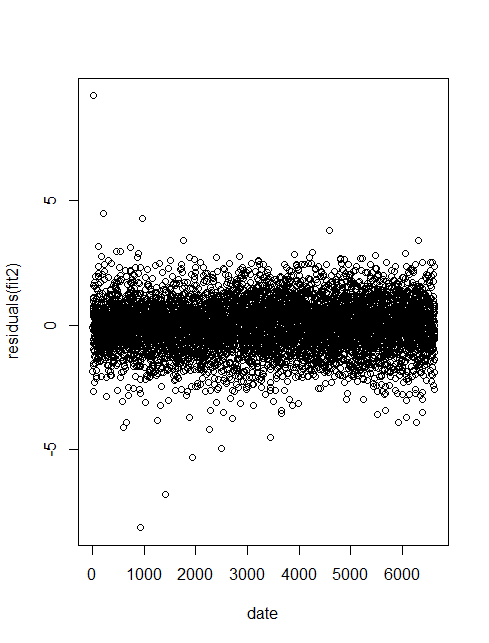
\includegraphics[width=8cm,height=6cm]{NYSE_res2.png}
\end {figure}
\noindent According to the figure, we can see that there is no ARCH effect in GARCH residual, we examine it with a test:
\begin{verbatim}
> ArchTest(residuals(fit2))
ARCH LM-test; Null hypothesis: no ARCH effects
data:  residuals(fit2)
Chi-squared = 5.5145, df = 12, p-value = 0.9386
\end{verbatim}
\noindent Hence we can trust there is no ARCH effect. Hence GARCH(1,1) model is predictive to the risk of stock market. With GARCH(1,1) we can predict when high risk happens and then avoid it.\\
\\
\textbf{Remark}:
In fact, it is not every GARCH(p,q) that works well, for example, the residuals of GARCH(2,2) model is:
\begin {figure}[h]
\centering
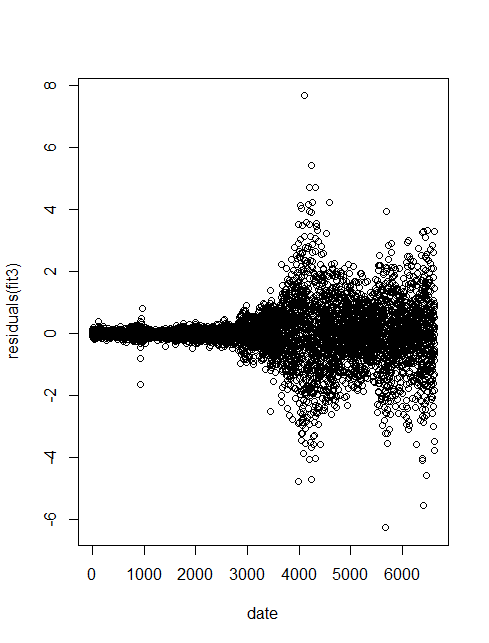
\includegraphics[width=8cm,height=6cm]{NYSE_res3.png}
\end {figure}
\noindent It is obvious that there is ARCH effect in residual of GARCH(2,2), hence GARCH(2,2) can not help us to avoid high risk in stock exchange.


\end{document} 